\chapter{Аналитический раздел}

В данном разделе будут выдвинуты требования к приложению, определены пользователи системы, формализованы хранимые о системе данные, а также проведен анализ существующих решений и выбор модели базы данных.

\section{Требования к приложению}

Приложение должно поддерживать определенный функционал:
\begin{itemize}
	\item персонализация пользователей;
	\item создание новых заявок и изменение информации об уже существующих;
	\item добавление оборудования;
	\item добавление навыков и отправка их на подтверждение;
	\item пополнение списка ролей конкретного пользователя и переключение между ними.
\end{itemize}

\section{Пользователи системы}

Для работы с системой обязательным этапом является прохождение персонализации. Пользователь может работать в системе под одной из следующих ролей.
\begin{enumerate}
	\item Оформитель -- пользователь, обладающий возможностями создания заявки, изменения ее параметров, закрытия заявки.
	\item Исполнитель -- пользователь, обладающий возможностями отправления своих навыков на подтверждение, взятия заявок на исполнение и их последующего закрытия.
	\item Администратор -- пользователь, обладающий возможностью подтверждения роли других администраторов и профессиональных навыков исполнителей.
\end{enumerate}
В ходе использования приложения предусмотрена возможность смены ролей.
На рисунке \ref{use-case} представлена диаграмма использования приложения.

\begin{figure}[H]
	\begin{center}
		%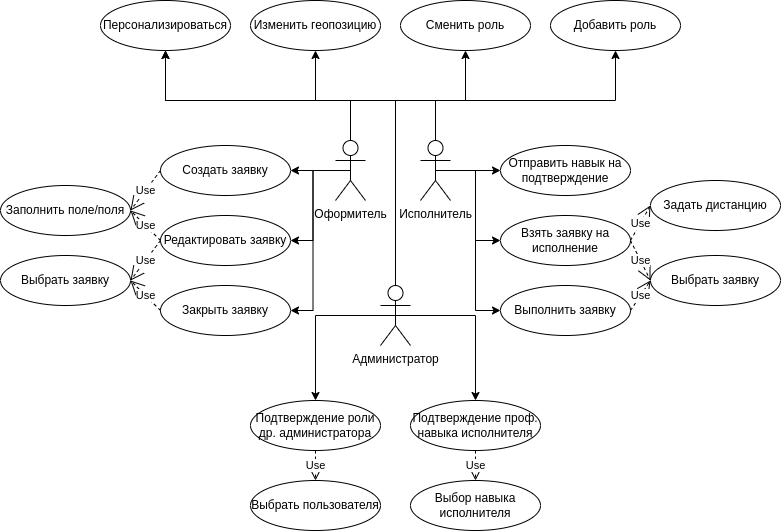
\includegraphics[scale=0.6]{assets/use-case.png}
		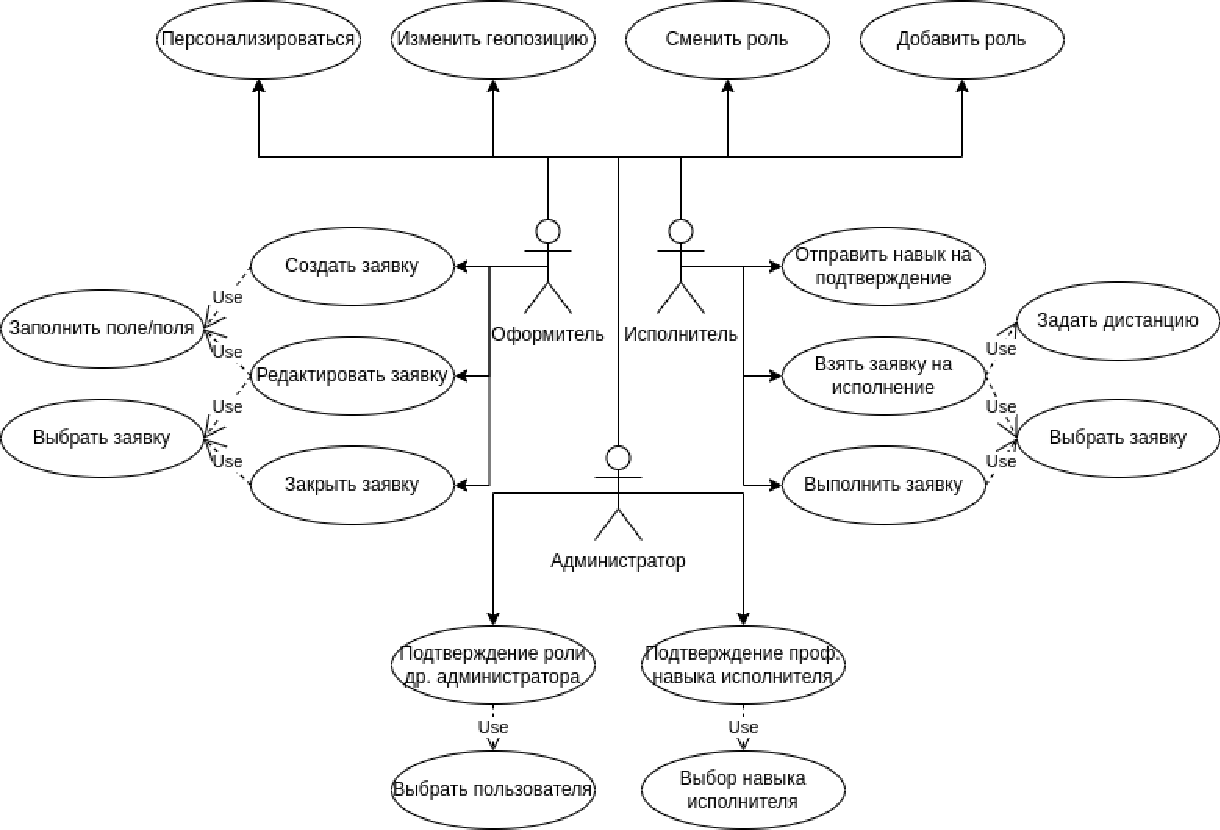
\includegraphics[page=1,scale=0.8]{assets/use-case.pdf}
		%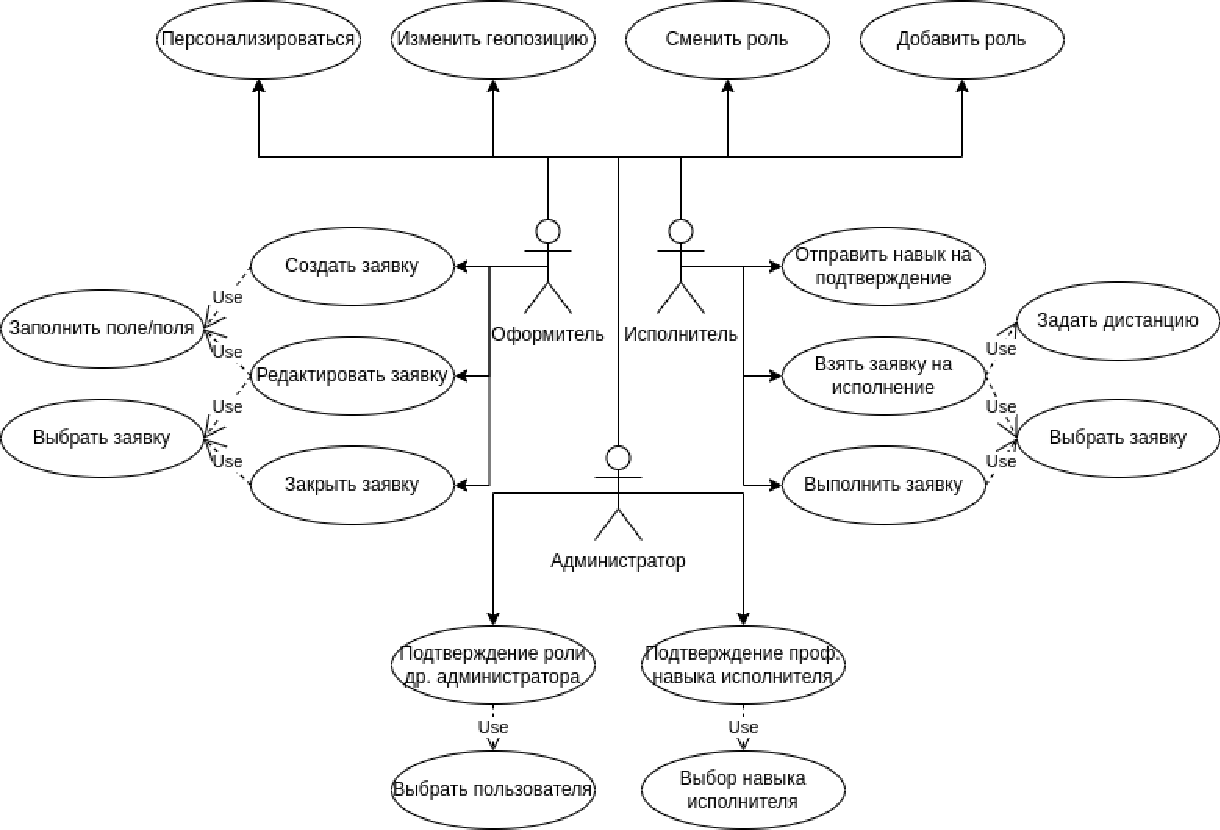
\includepdf[pages={1}, scale=0.6, offset=0cm 2cm]{assets/use-case.pdf}
	\end{center}
	\caption{Use-case диаграмма}
	\label{use-case}
\end{figure}

\section{Формализация данных}

База данных состоит из нескольких таблиц:
\begin{itemize}
	\item таблица пользователей User;
	\item таблица подключений Connection;
	\item таблица заявок Request;
	\item таблица оборудования Equipment;
	\item таблица навыков Skill;
	\item таблица подтверждения навыков исполнителей ExecutorSkill;
	%\item таблица, реализующая связь <<многие ко многим>> для оборудования и навыка EquipmentSkill;
	\item таблица, хранящая набор данных для предотвращения использования ненормативной лексики Ban.
\end{itemize}
На рисунке \ref{er-chen} представлена ER-диаграмма сущностей в нотации Чена.

\begin{figure}[H]
	\begin{center}
		%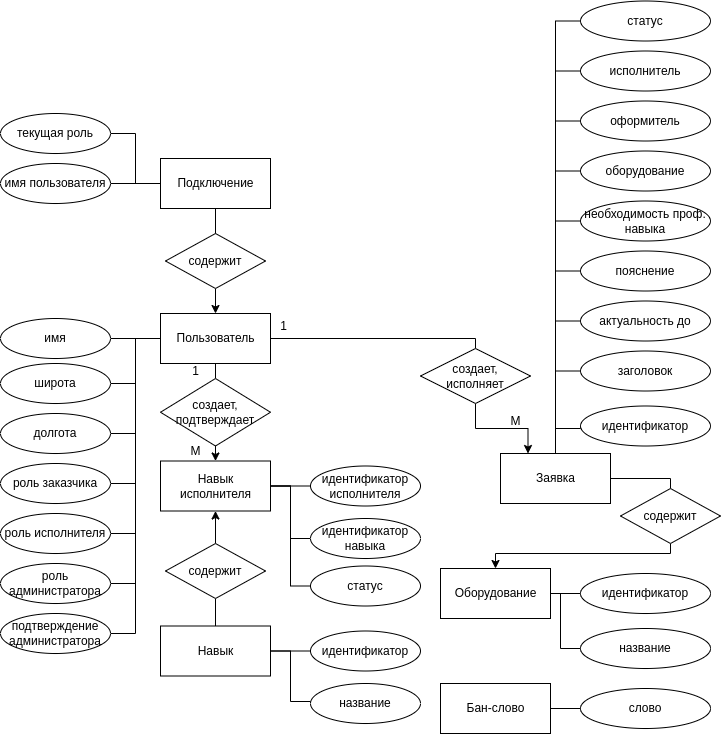
\includegraphics[scale=0.6]{assets/ER-Chen.png}
		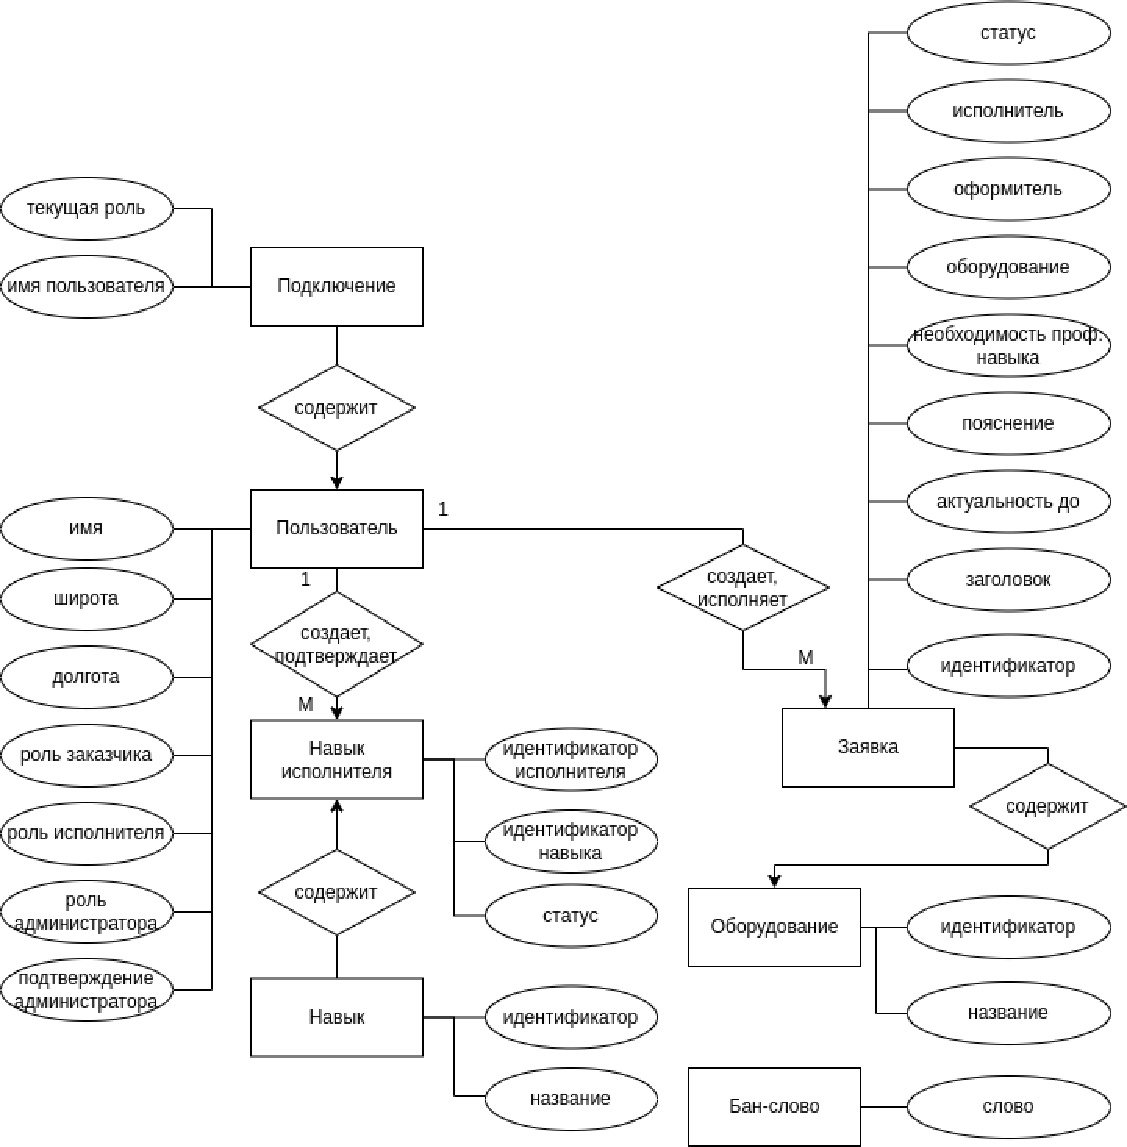
\includegraphics[page=1,scale=0.8]{assets/ER-Chen.pdf}
	\end{center}
	\caption{ER-диаграмма в нотации Чена}
	\label{er-chen}
\end{figure}

\section{Анализ существующих решений}

Среди уже имеющихся проектов, решающих поставленную задачу, были выделены 3 аналога (таблица \ref{decisions}) -- сервисы <<YouDo>> \cite{youdo}, <<Все соседи>> \cite{all_neighbour} и <<Привет, сосед!>> \cite{hello_neighbour}. Сравнение проводилось по ряду критериев, а именно авторизация, наличие территориальной привязки, охват аудитории, а также были выделены преимущественные особенности системы.

\begin{table}[H]
	\centering
	\caption{Существующие решения поставленной задачи}
	\label{decisions}
	\begin{tabular}{|p{2.3cm}|p{3.3cm}|p{3cm}|p{3cm}|p{3.1cm}|}
		\hline
		\textbf{Название проекта} & \textbf{Авторизация} & \textbf{Наличие территориальной привязки} & \textbf{Охват аудитории} & \textbf{Особенности системы}\\
		\hline 
		\textbf{YouDo} & Электронная почта или Вконтакте, Одноклассники, Google, Mail, Apple & На уровне города & Более 2.5 миллионов пользователей & Заказо- ориентирован- ность со стабильной системой отзывов\\
		\hline
		\textbf{Все соседи} & Номер телефона & Устанавлива- ется с точностью до дома & Около 60 тыс. пользователей & Бартерная система взаимовыручки\\
		\hline
		\textbf{Привет, сосед!} & Электронная почти или Вконтакте, Facebook, Одноклассники, Google, Yandex, Apple & Устанавлива- ется с точностью до дома & Около 2 тыс. пользователей & Уклон в социальную сеть с бонусной программой \\
		\hline
	\end{tabular}
\end{table}

Стоит упомянуть, что все вышеуказанные решения имеют мобильные версии для IOS и Android, а также Web-версии приложений.

У каждого вышеупомянутого аналога имеются недостатки среди выделенных критериев, как например слабоконкретизированная геопозиция, неудобная авторизация или малое количество участников. 

Создаваемый продукт должен не просто быть на уровне с конкурирующими платформами, но и предоставлять пользователям дополнительный функционал. Такими особенностями станут:
\begin{itemize}
	\item территориальная привязка на уровне геолокации;
	\item авторизация внутри мессенджера telegram, имеющего больший охват аудитории и возможность лично написать оформителю/исполнителю заявки;
	\item смена роли -- пользователь сможет не только создавать заявки, но и помогать другим, исполняя их, в рамках одного аккаунта;
	\item добавление навыков и оборудования -- для некоторых задач простого желания помочь недостаточно, а данный функционал поможет облегчить процесс выбора заявок для исполнения.;
	\item механизм предотвращения ненормативной лексики при создании заявок.
\end{itemize}

% Избавиться от первого из них не составляет труда (стоит повысить точность геолокации), тогда как последние два могут быть сведены к использованию популярного мессенджера, имеющего большой охват аудитории. Таким вариантом можно смело назвать telegram, который не уступает приведенным проектам в кроссплатформенности.

\section*{Анализ моделей баз данных}

Модель данных -- это совокупность правил порождения структур данных в базе
данных, операций над ними, а также ограничений целостности, определяющих
допустимые связи и значения данных, последовательность их изменения \cite{db}.

В настоящее время разработано множество моделей данных, рассмотрим основные из них.

\subsection{Иерархическая модель данных}

Иерархическая модель данных подразумевает что элементы, организованные в структуры, объединены иерархической или древовидной связью. В таком представлении родительский элемент может иметь несколько дочерних, а дочерний -- только один родительский.

Каждая вершина дерева соответствует типу сущности ПО.  Конечные вершины, то есть вершины, из которых не выходит ни одной дуги, называются листьями дерева. Каждая некорневая вершина связана с родительской вершиной иерархическим групповым отношением. Тип сущности характеризуется произвольным количеством атрибутов, связанных с ней отношением 1:1. Атрибуты, связанные с сущностью отношением 1:n, образуют отдельную сущность (сегмент) и переносятся на следующий уровень иерархии. Реализация связей типа n:m не поддерживается.

В иерархической модели не может быть сегментов, не связанных с вершинами верхнего уровня (кроме корневой). Добраться до нужной записи можно только пройдя по всему дереву сущностей и по записям текущего сегмента, так как связи между записями обычно выполнены в виде ссылок. Каждая из записей идентифицируется по полному сцепленному ключу, который в свою очередь является конкатенированным значением идентификаторов сегментов, через которые осуществляется доступ, и идентификатором самой записи. 

Существенным недостатком такой модели является то, что каждая сущность может относится только к одному родительскому сегменту. Таким образом при необходимости множественного отношения происходит дублирование данных, что может привести к нарушению логической целостности БД.

\subsection{Сетевая модель данных}

Сетевая модель базы данных подразумевает, что у родительского элемента может быть несколько потомков, а у дочернего элемента -- несколько предков. Структура такой модели представлена в виде графа, причем каждая вершина графа хранит экземпляры сущностей (записи одного типа) и сведения о групповых отношениях с сущностями других типов. Каждая запись может хранить произвольное количество значений атрибутов (элементов данных и агрегатов), характеризующих экземпляр сущности. Для каждого типа записи выделяется первичный ключ – атрибут, значение которого позволяет однозначно идентифицировать запись среди экземпляров записей данного типа.

Связи между записями выполняются в виде указателей, т.е. каждая запись хранит ссылку на другую однотипную запись (или признак конца списка) и ссылки на списки подчинённых записей, связанных с ней групповыми отношениями. Таким образом, в каждой вершине записи хранятся в виде связного списка.

В этой модели связь 1:n между сущностями реализуется с помощью групповых отношений, а связи 1:n между атрибутами сущности -- в рамках записи. Для реализации связей типа n:m вводится вспомогательный тип записи и две связи 1:n. 

Физическая независимость не обеспечивается в сетевой модели данных, потому что наборы организованы с помощью физических ссылок. Помимо этого данная модель не обеспечивает независимость данных от программ. Эти недостатки помешали обрести ей широкое распространение из-за сложного проектирования и поддержки.

\subsection{Реляционная модель данных}

Реляционная модель данных является самой распространенной в использовании. В отличие от вышеописанных, в данной модели не существует физических отношений между сущностями. Хранение информации осуществляется в виде таблиц (отношений), состоящих из рядов и столбцов. Отношение имеет имя, которое отличает его от имён всех других отношений. Атрибутам реляционного отношения назначаются имена, уникальные в рамках отношения. Обращение к отношению происходит по его имени, а к атрибуту – по именам отношения и атрибута.

В реляционных моделях данных нет необходимости просматривать все указатели, что облегчает выполнение запросов на выборку информации по сравнению с сетевыми и иерархическими моделями. Это означает, что порядок записей не является важным, также как и порядок столбцов.

Каждая запись идентифицируется уникальной комбинацией атрибутов -- первичным ключом. Для связи между отношениями используется внешний ключ -- копия первичного или уникального ключа атрибута сторонней сущности. Таким образом можно реализовывать связь 1:n. Для обеспечения связи n:m вводится дополнительная сущность, атрибутами которой являются внешние ключи соответствующих сущностей.

Обработка данных осуществляется с помощью декларативного языка запросов SQL \cite{sql}. 

% Так как хранение осуществляется в виде двумерных таблиц, реализация сложных структур является невозможной.

\section{Выбор модели базы данных}

В данном проекте будет использоваться реляционная модель данных, потому что в рамках проекта она обладает следующими преимуществами:
\begin{itemize}
	\item изложение информации осуществляется с помощью простых и понятных форм (таблиц);
	\item позволяет работать со структурированными данными, структура которых не подвергается частым изменениям;
	\item имеет возможность произвольного доступа к записям сущностей;
	\item исключает дублирование, реализуя связь между отношениями посредством внешнего ключа.
\end{itemize}

\section{Вывод из раздела}

В данном разделе были выделены ролевые модели системы, конкретизированы хранимые данные и их связь между собой, построены соответствующие диаграммы. Также был проведен анализ существующих на рынке решений, который позволил понять, какие особенности стоит добавить в разрабатываемый проект. Был осуществлен выбор модели базы данных.